\chapter{Supplementary material}
\vspace{-1cm}

\section{SOC: other figures}
\label{ch:SM_SOC}
The following two figures report some analysis of the duration of each avalanche for the sandpile model described in \ref{ch:SOC}. The duration is here operationally defined as the number of times the queue of unstable nodes has been updated, i.e. the number of times a toppling event leads to other sites being unstable. 
\begin{figure}[h] 
    \centering
    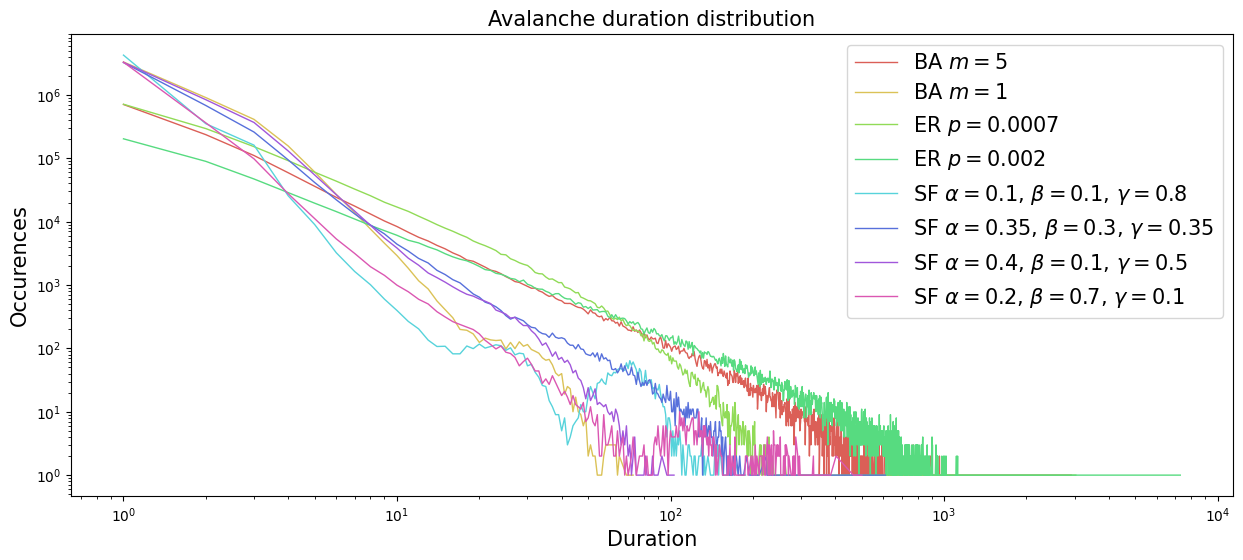
\includegraphics[width=0.9\textwidth]{images/task15/d_dist2.png} 
    \vspace{-0.5cm}
    \caption{Distribution of the duration of each avalanche.}
    \label{fig:adist} 
\end{figure}

\begin{figure}[h] 
    \centering
    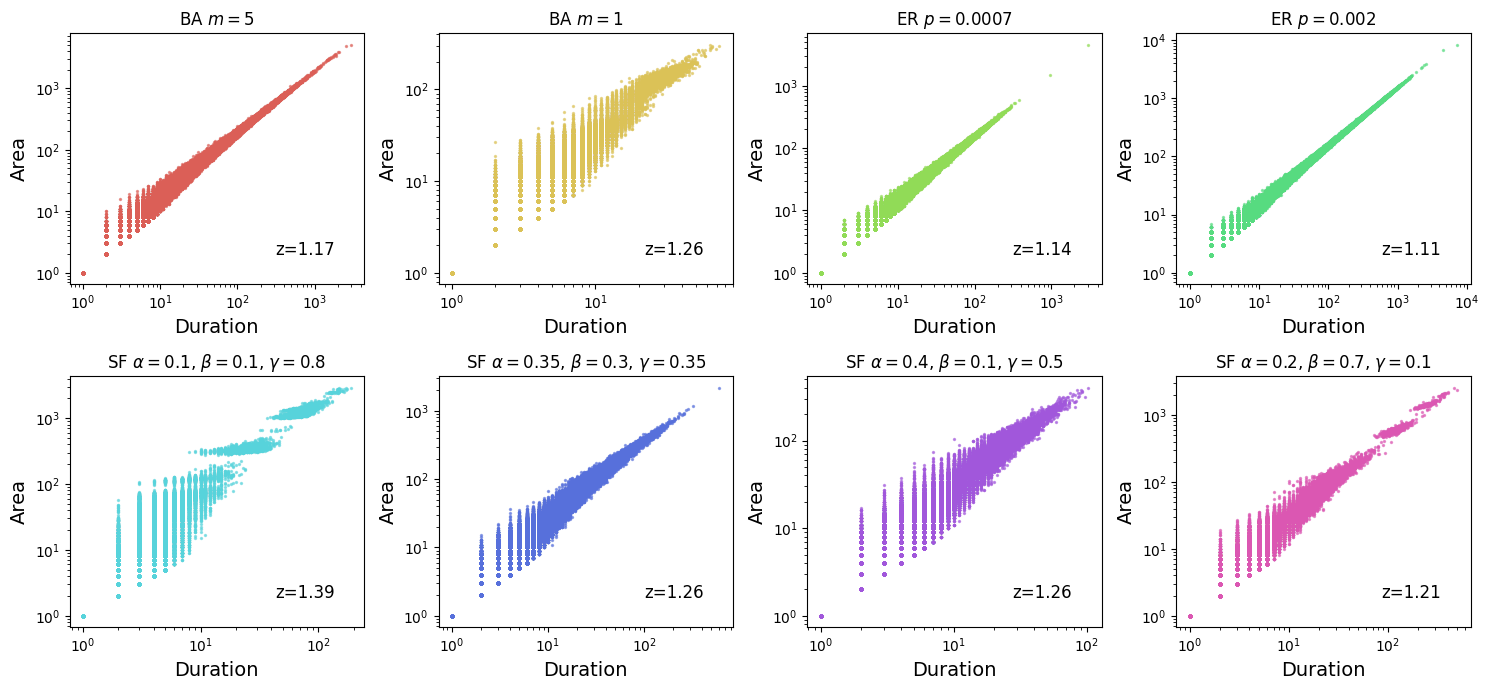
\includegraphics[width=1\textwidth]{images/task15/at.png} 
    \vspace{-0.5cm}
    \caption{Relation between the avalanche area and the duration of the cascade.}
    \label{fig:adist} 
\end{figure}

\section{SOC: interdependent networks}
\label{ch:SM_SOC2}
I simulated the sandpile dynamics over a coupled $R(3)$-$B(p)$-$R(3)$ networks, as described in \cite{brummitt2012suppressing}. Each network is a $z=3$ regular graph with $N=2\times 10^3$ nodes. The coupling is achieved by selecting uniformly at random $l$ nodes from each network with probability $p$ and connecting the correspondent edge stubs. For each value of $p$, eight independent realizations have been analyzed. \\
The simulations last $5 \times 10^7$ iterations with a dissipation rate $f=0.01$. \\
Even with this simplified analysis, one can appreciate the minimum in the number of large avalanches in network $a$, obtained by tuning the coupling probability around $p=0.07$. 

\begin{figure}[h]
    \centering
    \begin{minipage}{0.5\textwidth}
        \centering
        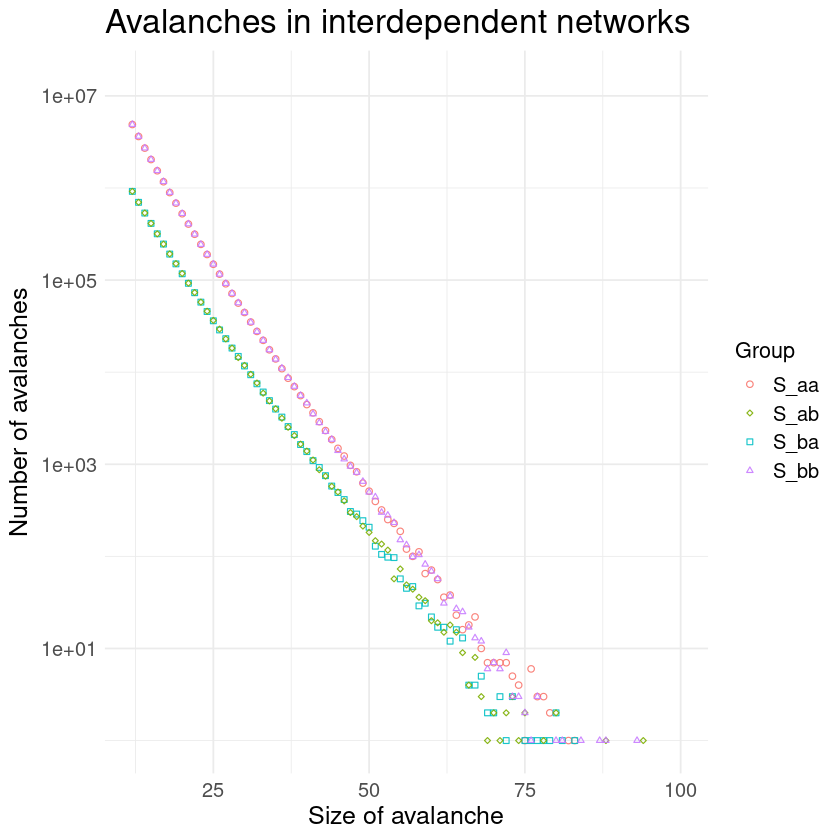
\includegraphics[width=\textwidth]{images/task15/coupled2.png}
        %\caption{Caption for the first figure}
    \end{minipage}\hfill
    \begin{minipage}{0.5\textwidth}
        \centering
        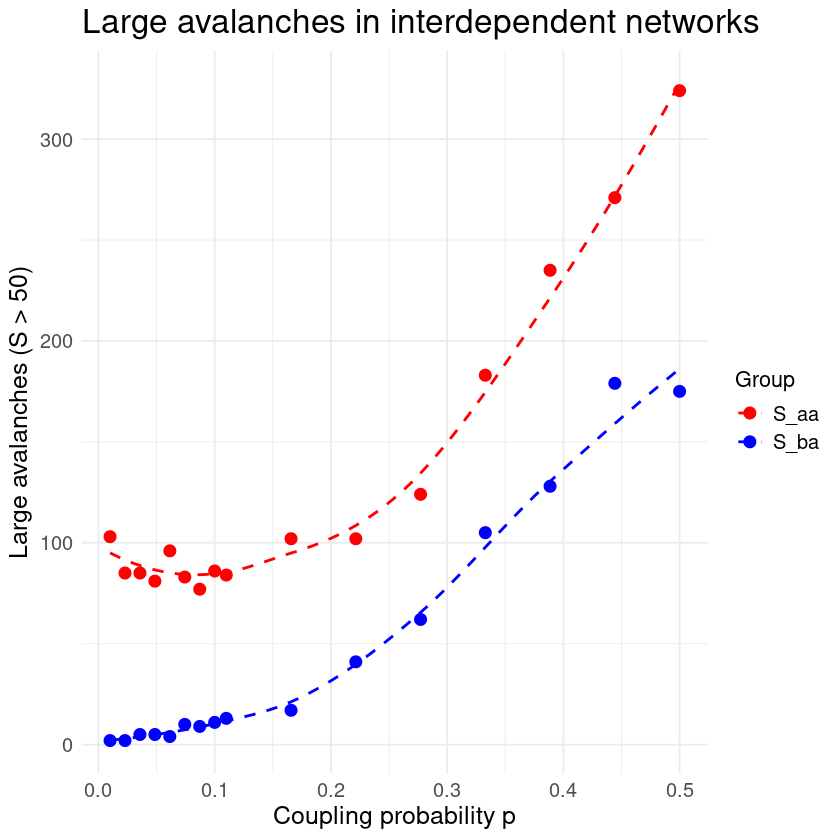
\includegraphics[width=\textwidth]{images/task15/coupled1.png}
        %\caption{Caption for the second figure}
    \end{minipage}
    \caption{(left) The avalanche size distribution in interdependent networks. Only values for $S>10$ are shown.  (right) Number of large avalanches ($S>50$) in network $a$ as a function of the coupling probability $p$. $S\_aa$ and $S\_ba$ refer to avalanches started in network $a$ and $b$ respectively.}
    \label{fig:figures}
\end{figure}

\newpage

\section{Axelrod's model: other figures}
\label{ch:sm_culture}
The following section contains the figures regarding Axelrod's dynamics on top of all the networks analyzed in this report. The general analysis is reported in the main text (see chapter \ref{ch:culture}). Each network has $2\times10^3$ nodes and the results refer to $4$ independent simulations of $5\times10^7$ iterations each. 
\noindent Moreover, the dynamics have been tested also on top of a $L\times L$ lattice ($L=50$). The simulations last for $10^{10}$ iterations, repeated $3$ independent times. This numerical analysis should be compatible with the ones in the literature. 

\begin{figure}[h] 
    \centering
    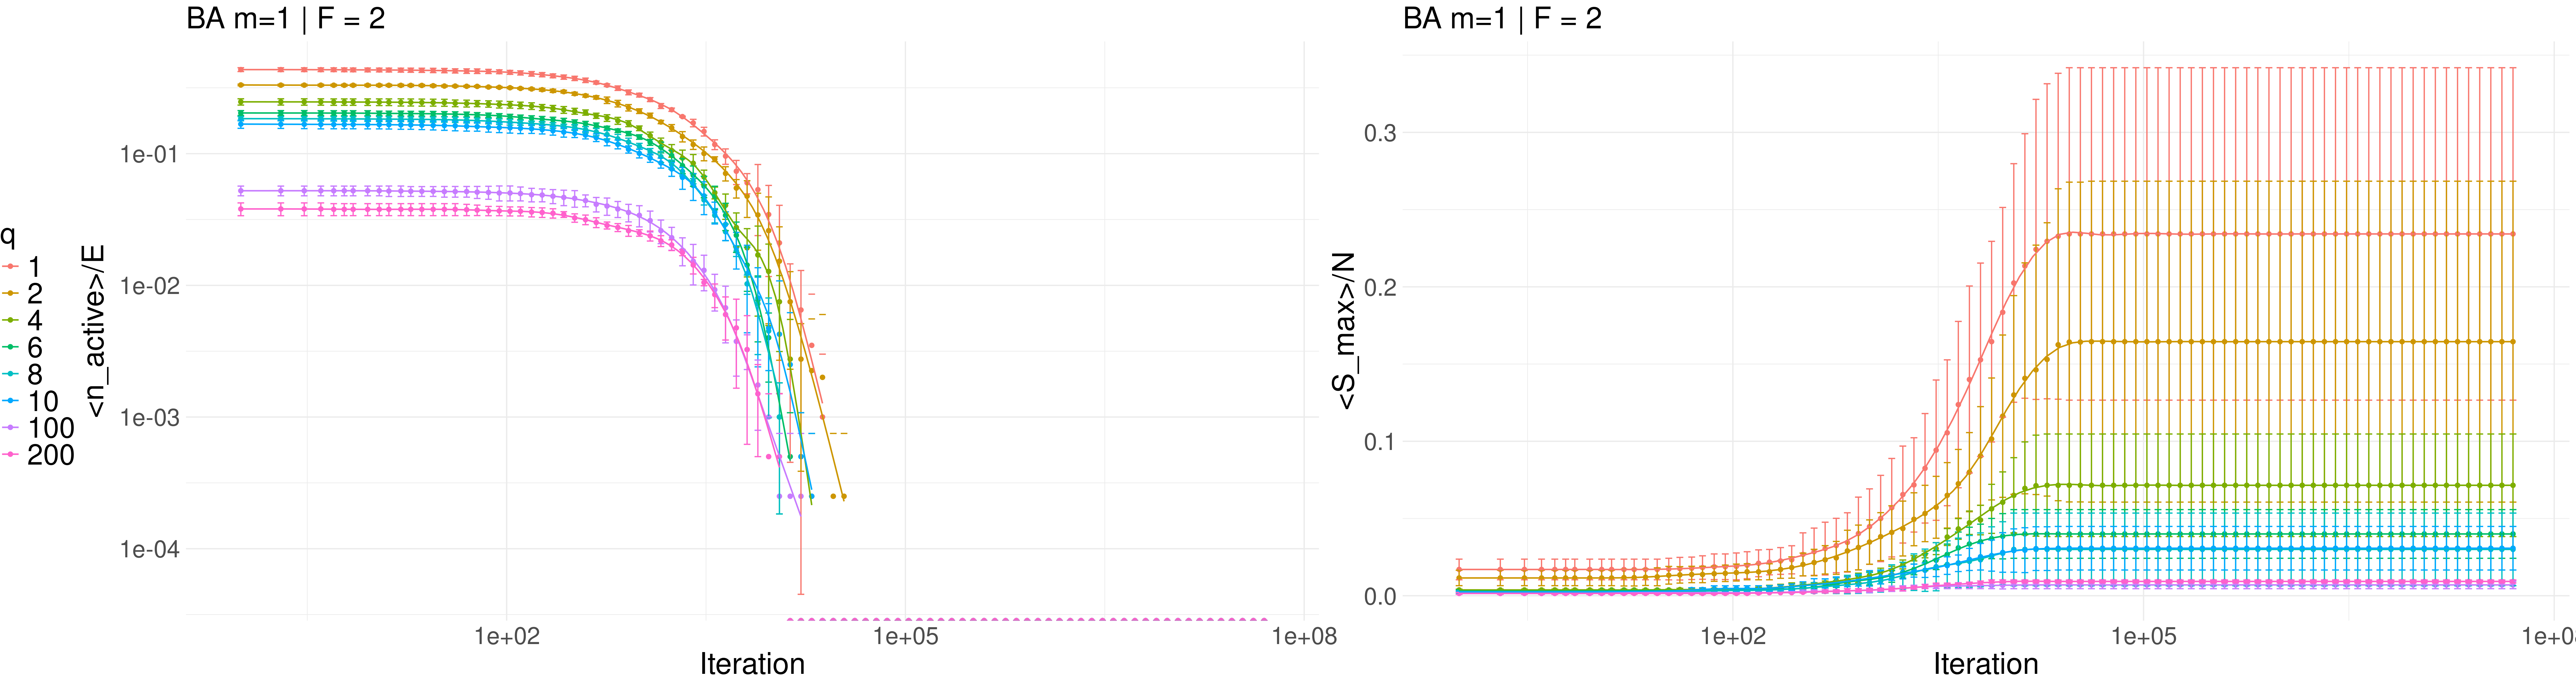
\includegraphics[width=1\textwidth]{images/task30/BA_1_2.png} 
    \vspace{-0.5cm}
    \caption{Barabasi-Albert with $m=1$. $F=2$.} 
\end{figure}

\begin{figure}[h] 
    \centering
    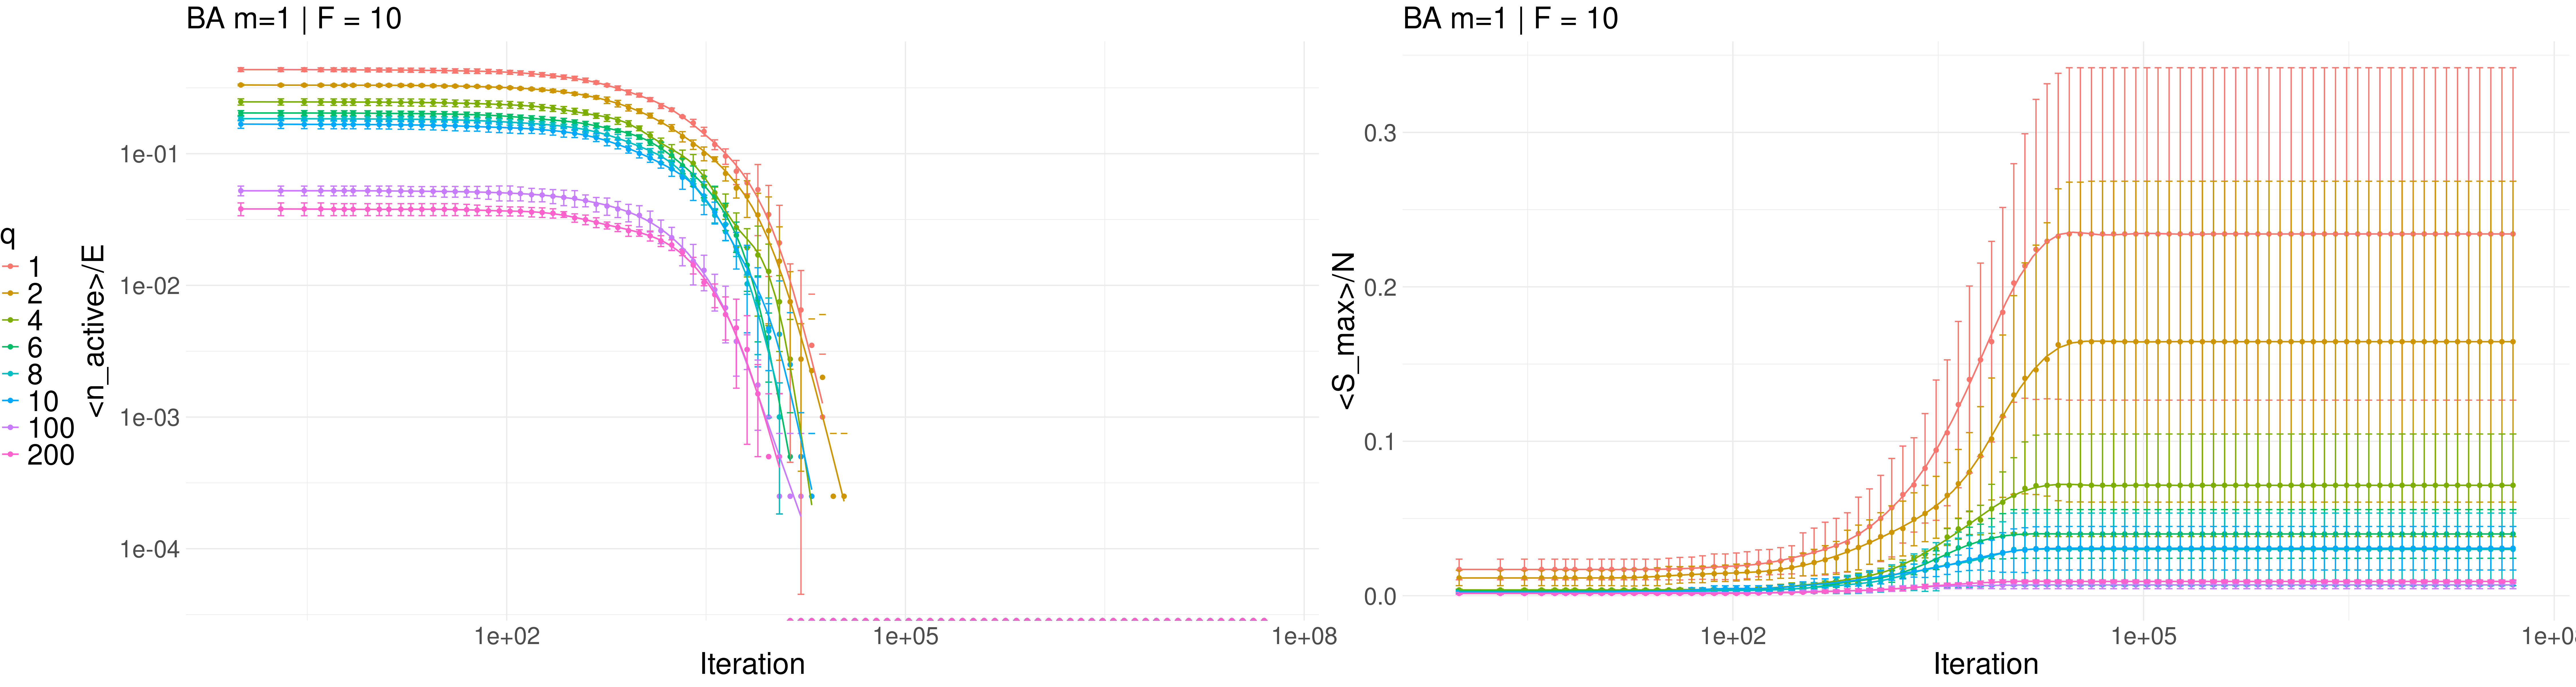
\includegraphics[width=1\textwidth]{images/task30/BA_1_10.png} 
    \vspace{-0.5cm}
    \caption{Barabasi-Albert with $m=1$. $F=10$.} 
\end{figure}


\begin{figure}[h] 
    \centering
    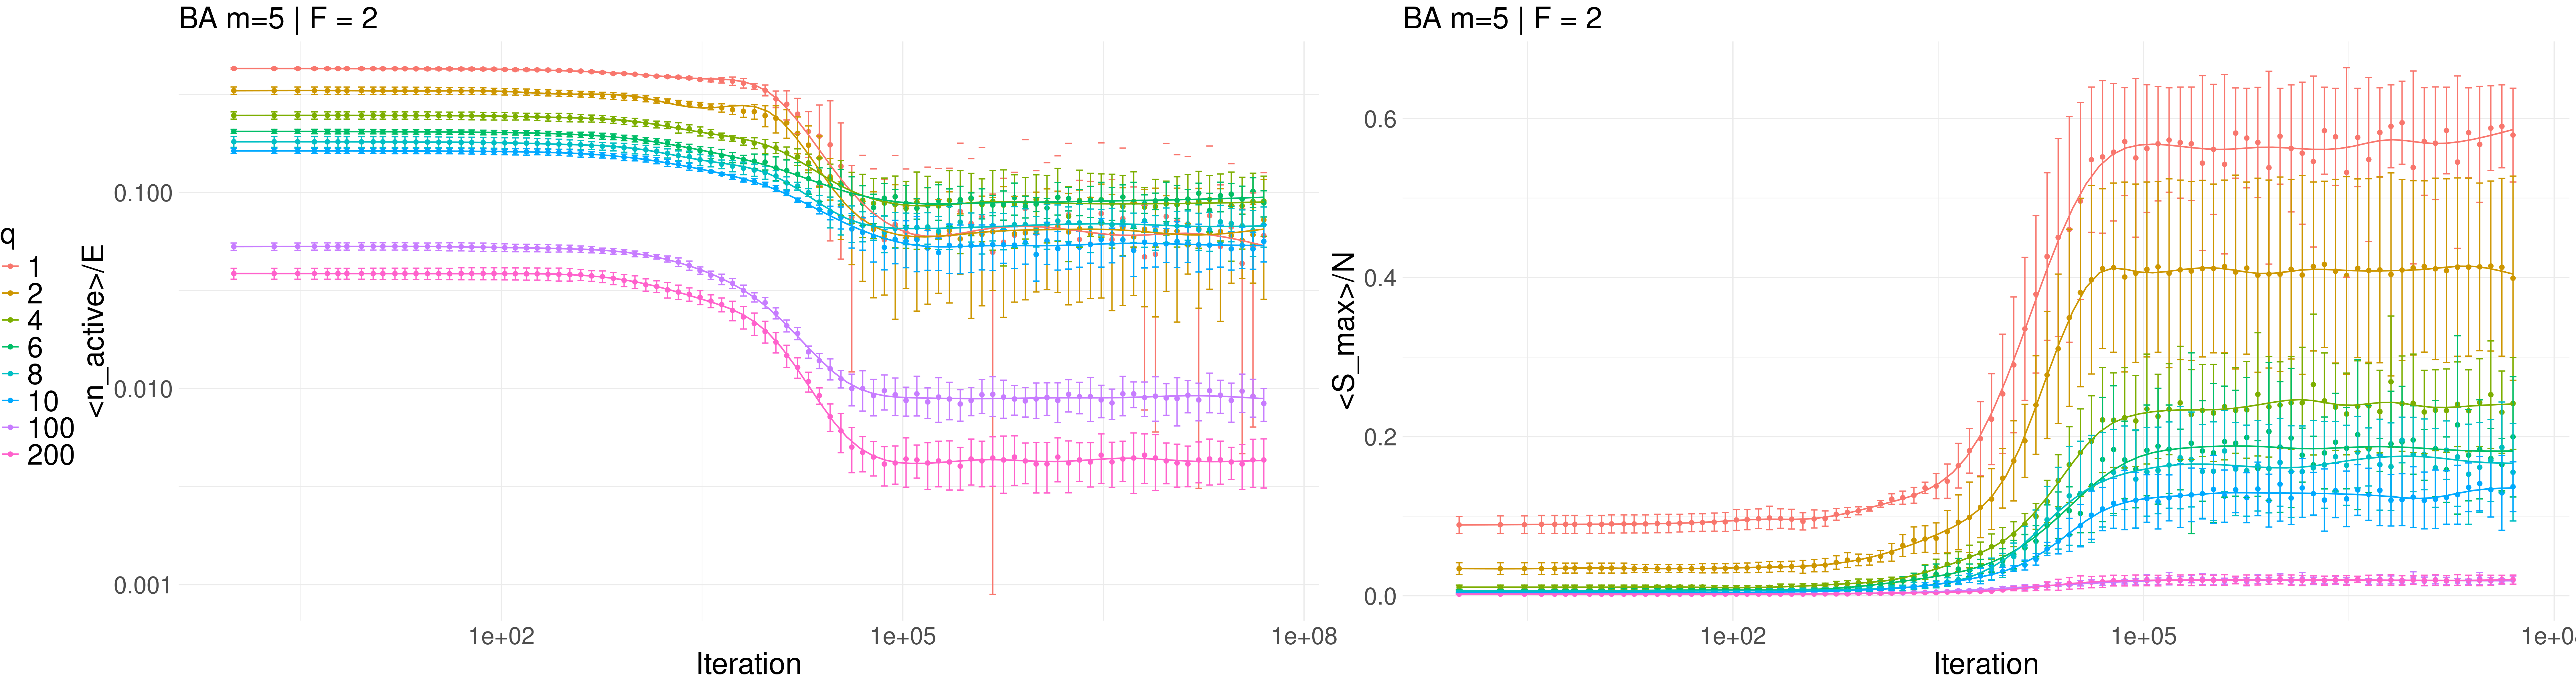
\includegraphics[width=1\textwidth]{images/task30/BA_5_2.png} 
    \vspace{-0.5cm}
    \caption{Barabasi-Albert with $m=5$. $F=2$.} 
\end{figure}

\begin{figure}[h] 
    \centering
    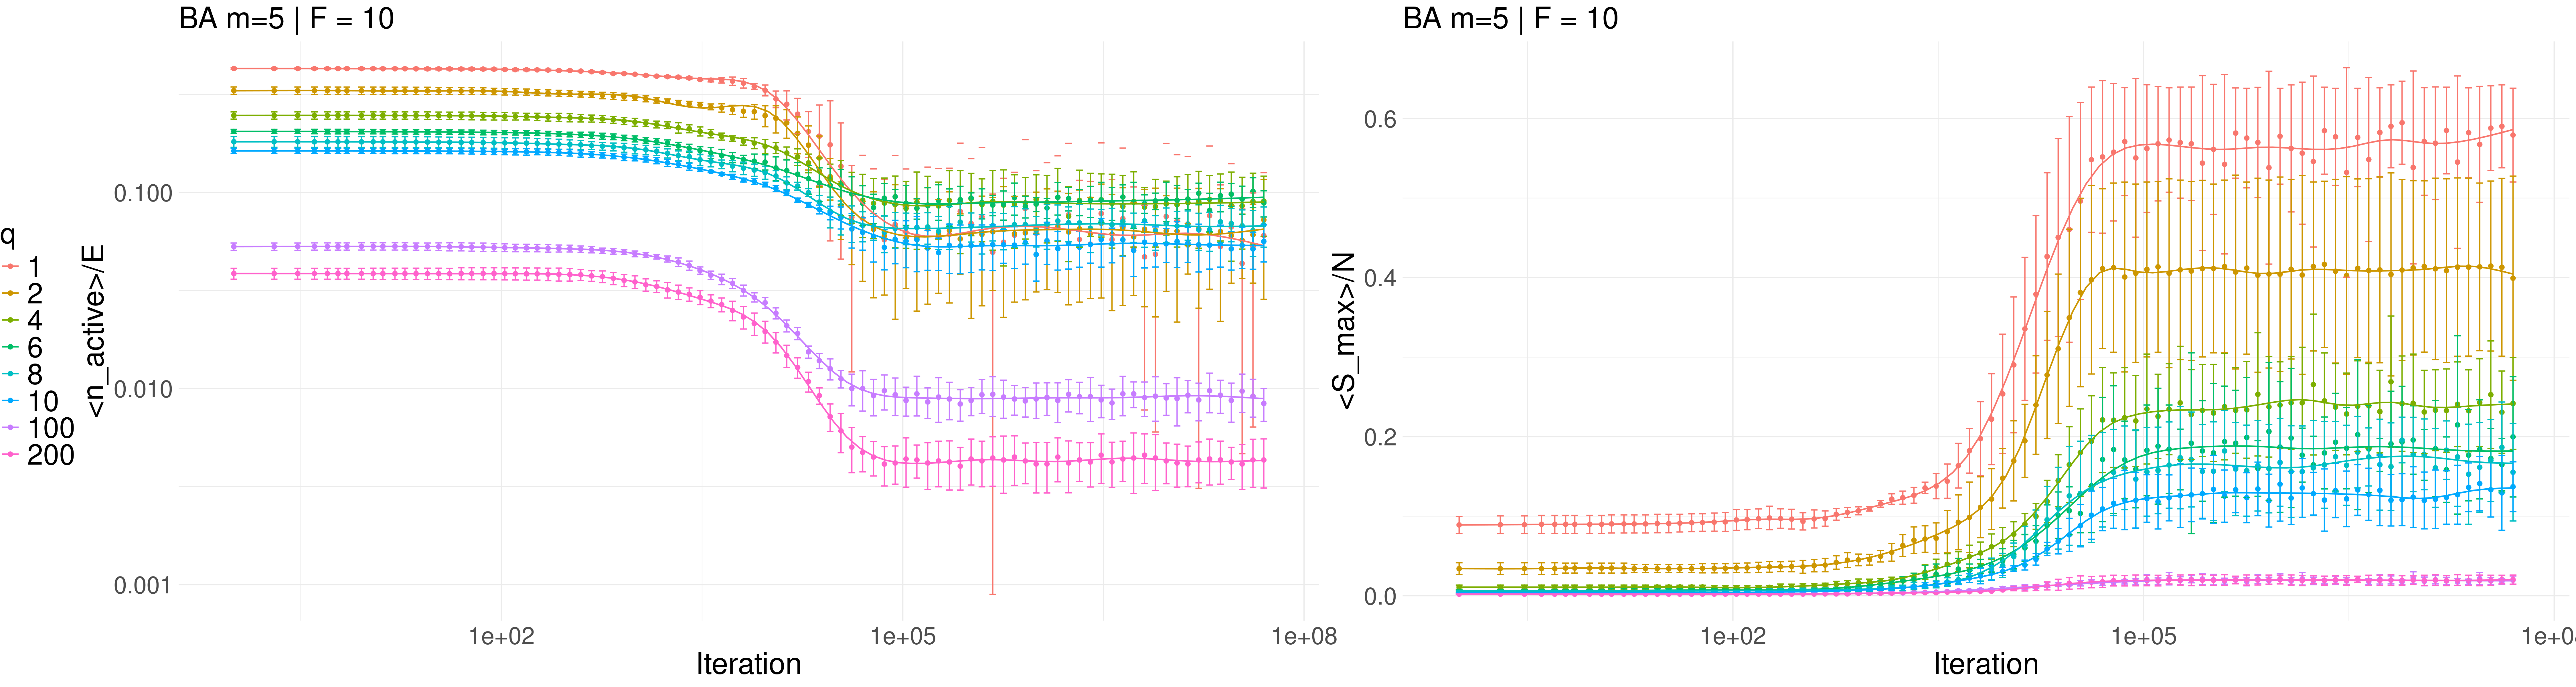
\includegraphics[width=1\textwidth]{images/task30/BA_5_10.png} 
    \vspace{-0.5cm}
    \caption{Barabasi-Albert with $m=5$. $F=10$.} 
\end{figure}

\begin{figure}[h] 
    \centering
    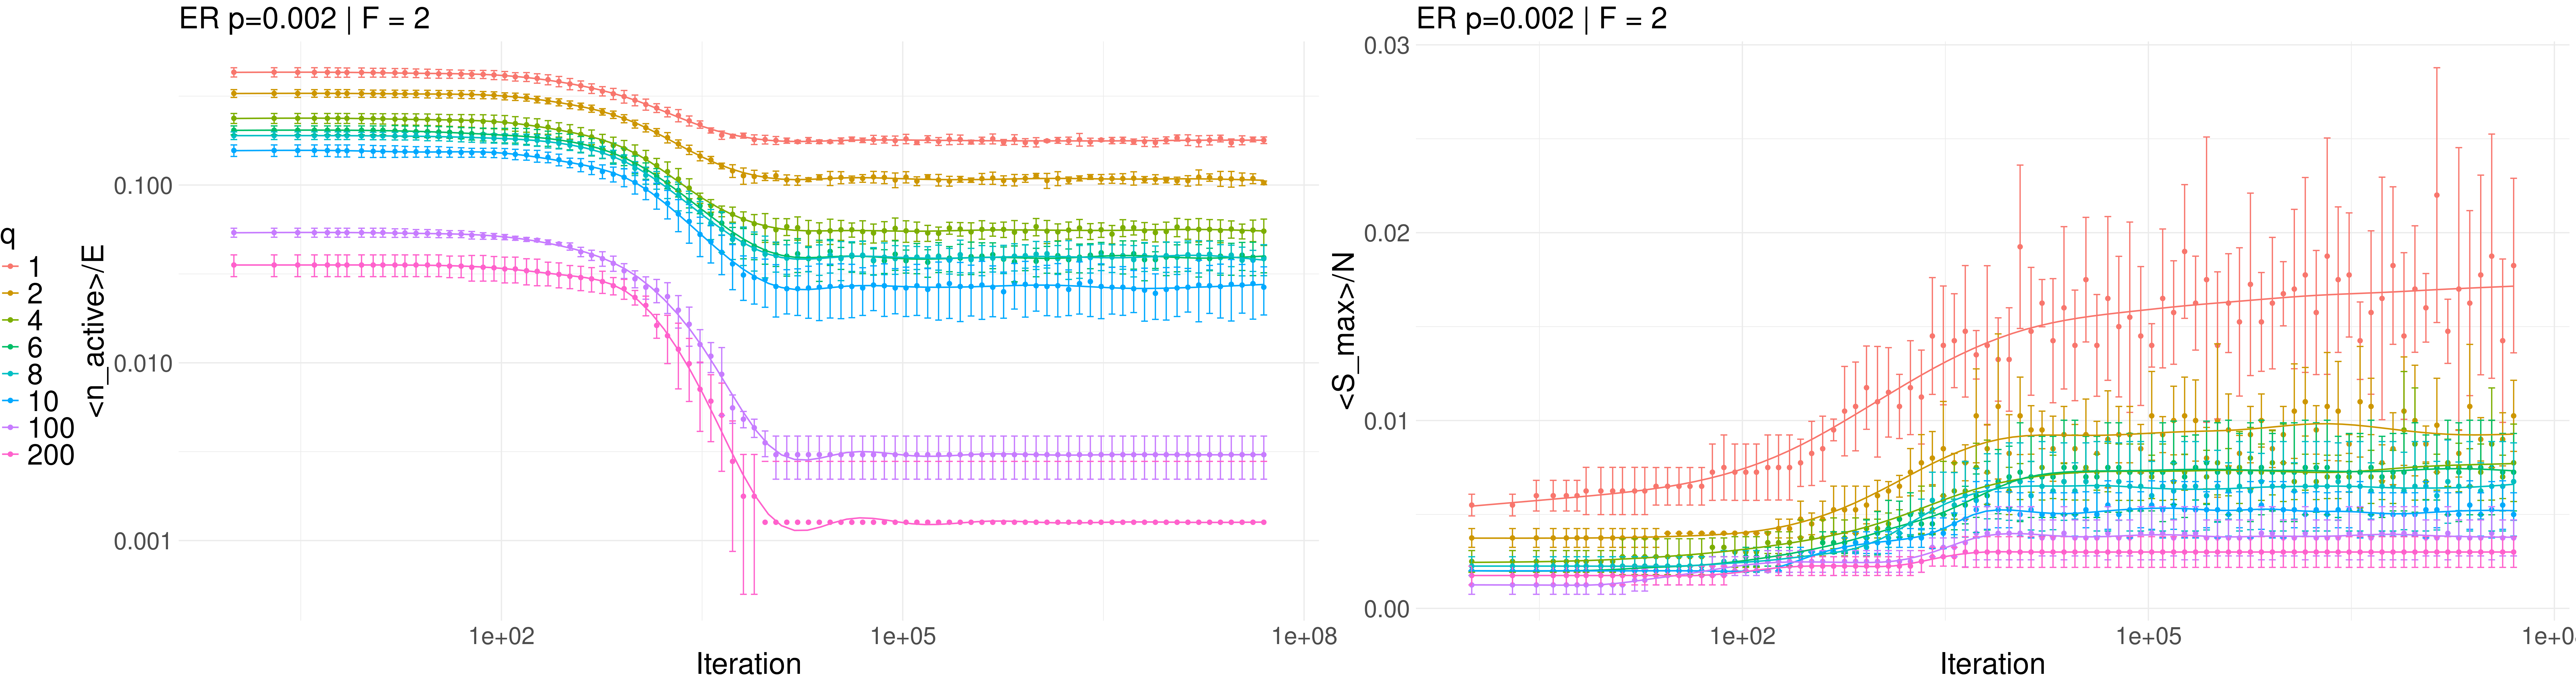
\includegraphics[width=1\textwidth]{images/task30/ER_0-002_2.png} 
    \vspace{-0.5cm}
    \caption{Erdős–Rényi with $p=2\times10^{-3}$. $F=2$.} 
\end{figure}


\begin{figure}[h] 
    \centering
    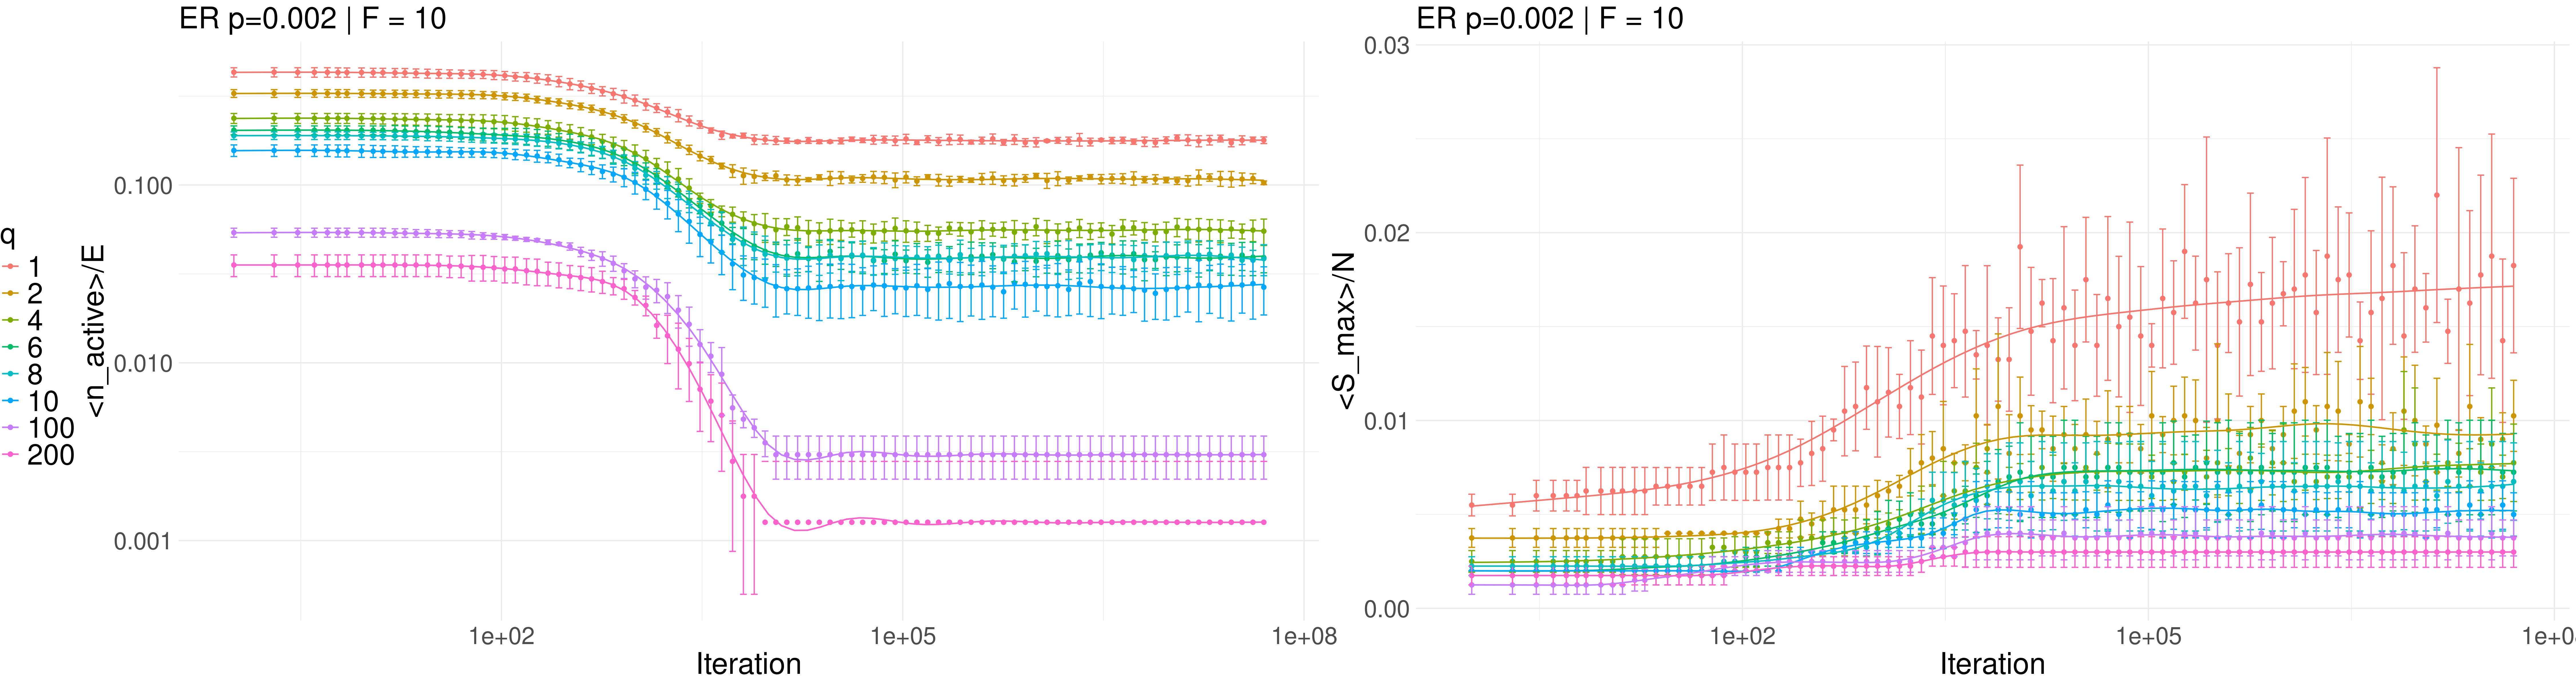
\includegraphics[width=1\textwidth]{images/task30/ER_0-002_10.png} 
    \vspace{-0.5cm}
    \caption{Erdős–Rényi with $p=2\times10^{-3}$. $F=10$.} 
\end{figure}


\begin{figure}[h] 
    \centering
    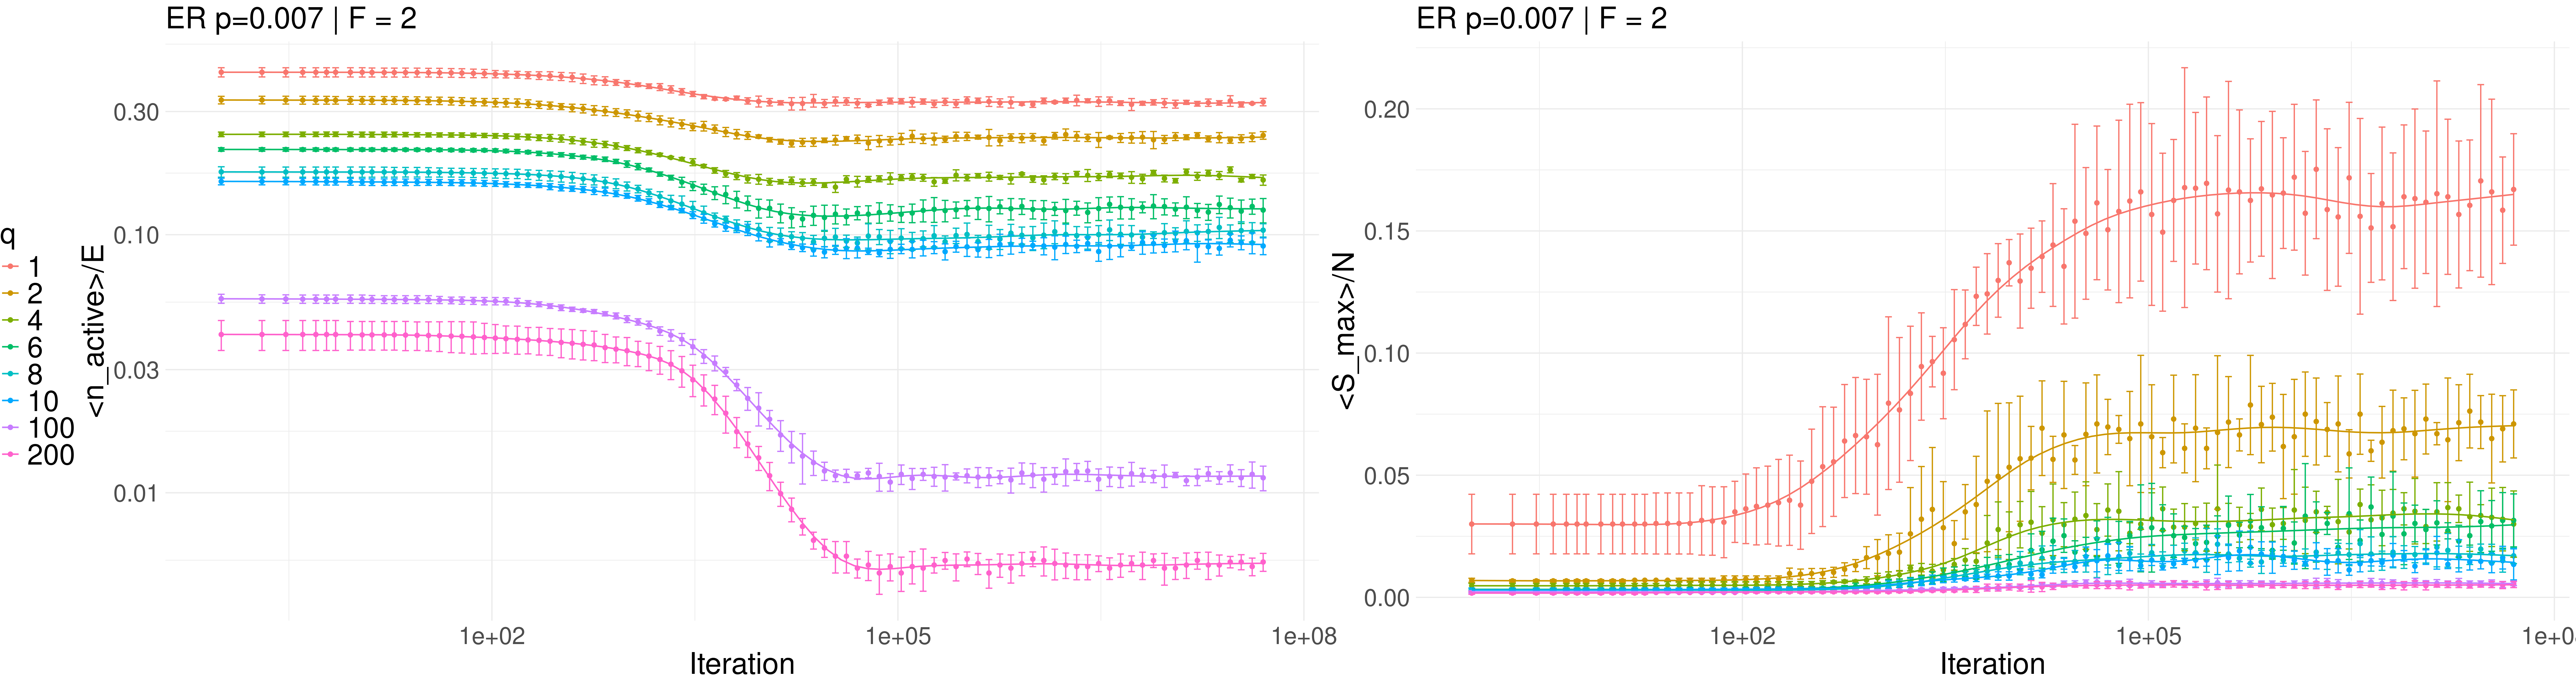
\includegraphics[width=1\textwidth]{images/task30/ER_0-007_2.png} 
    \vspace{-0.5cm}
    \caption{Erdős–Rényi with $p=7\times10^{-3}$. $F=2$.} 
\end{figure}


\begin{figure}[h] 
    \centering
    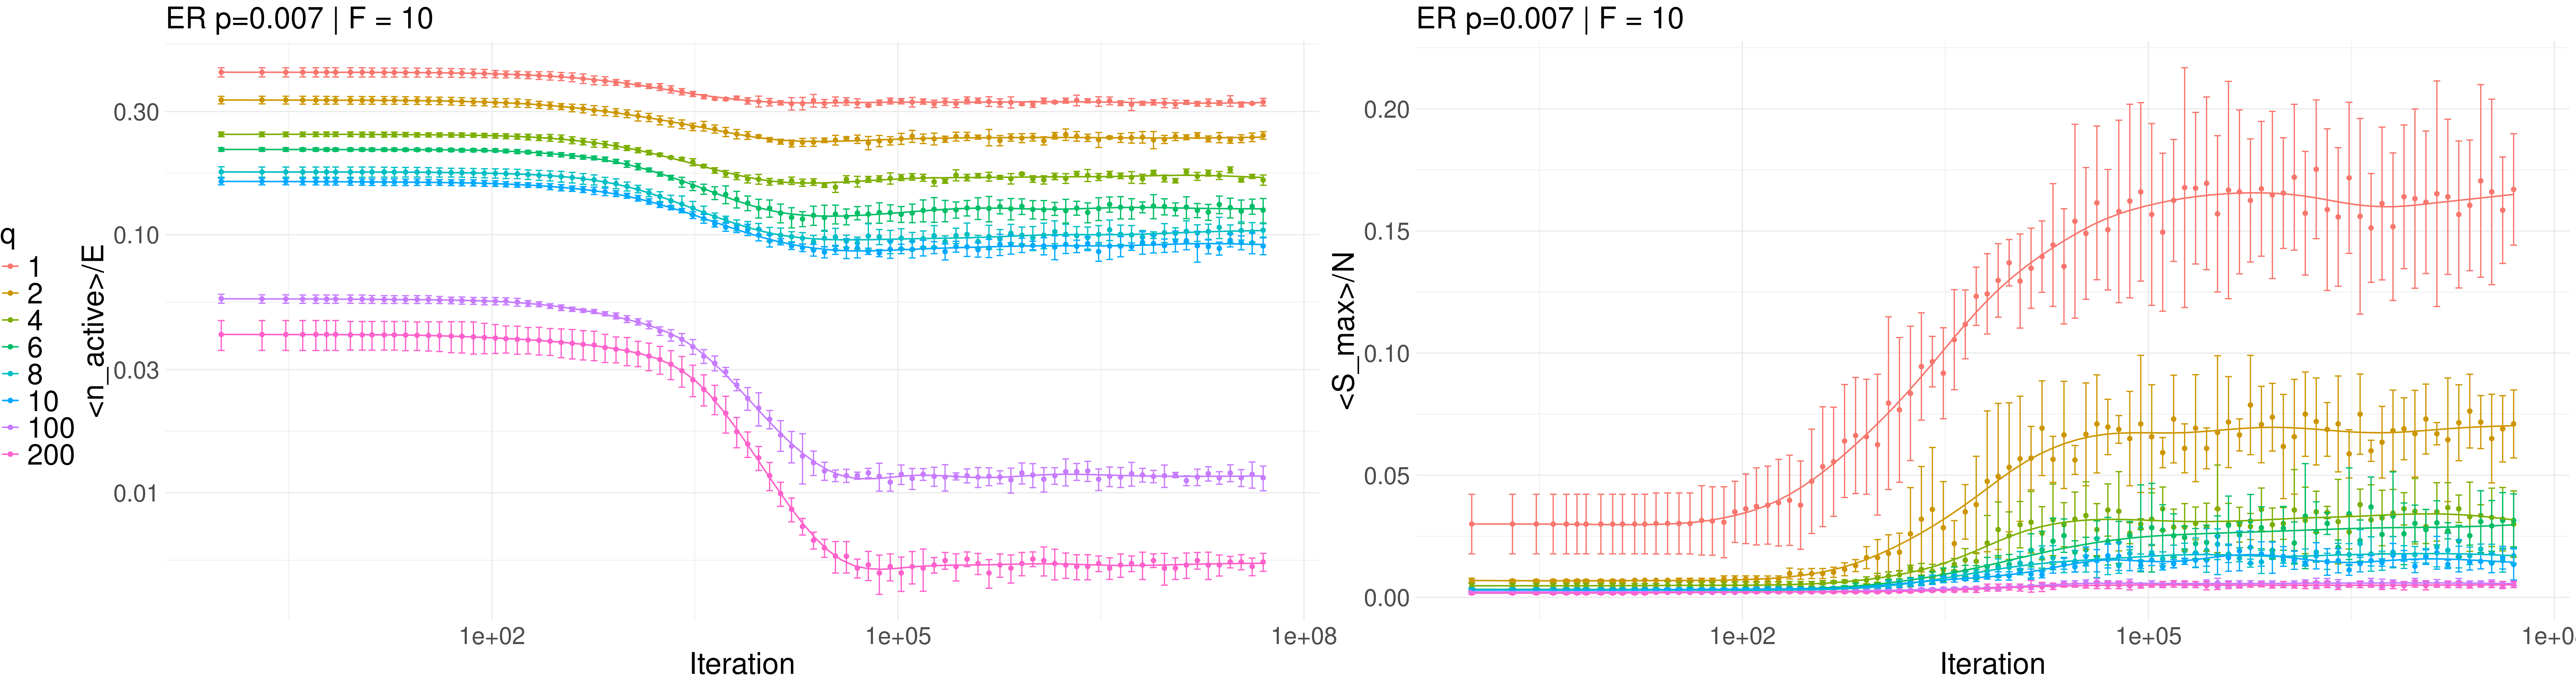
\includegraphics[width=1\textwidth]{images/task30/ER_0-007_10.png} 
    \vspace{-0.5cm}
    \caption{Erdős–Rényi with $p=7\times10^{-3}$. $F=10$.} 
\end{figure}


\begin{figure}[h] 
    \centering
    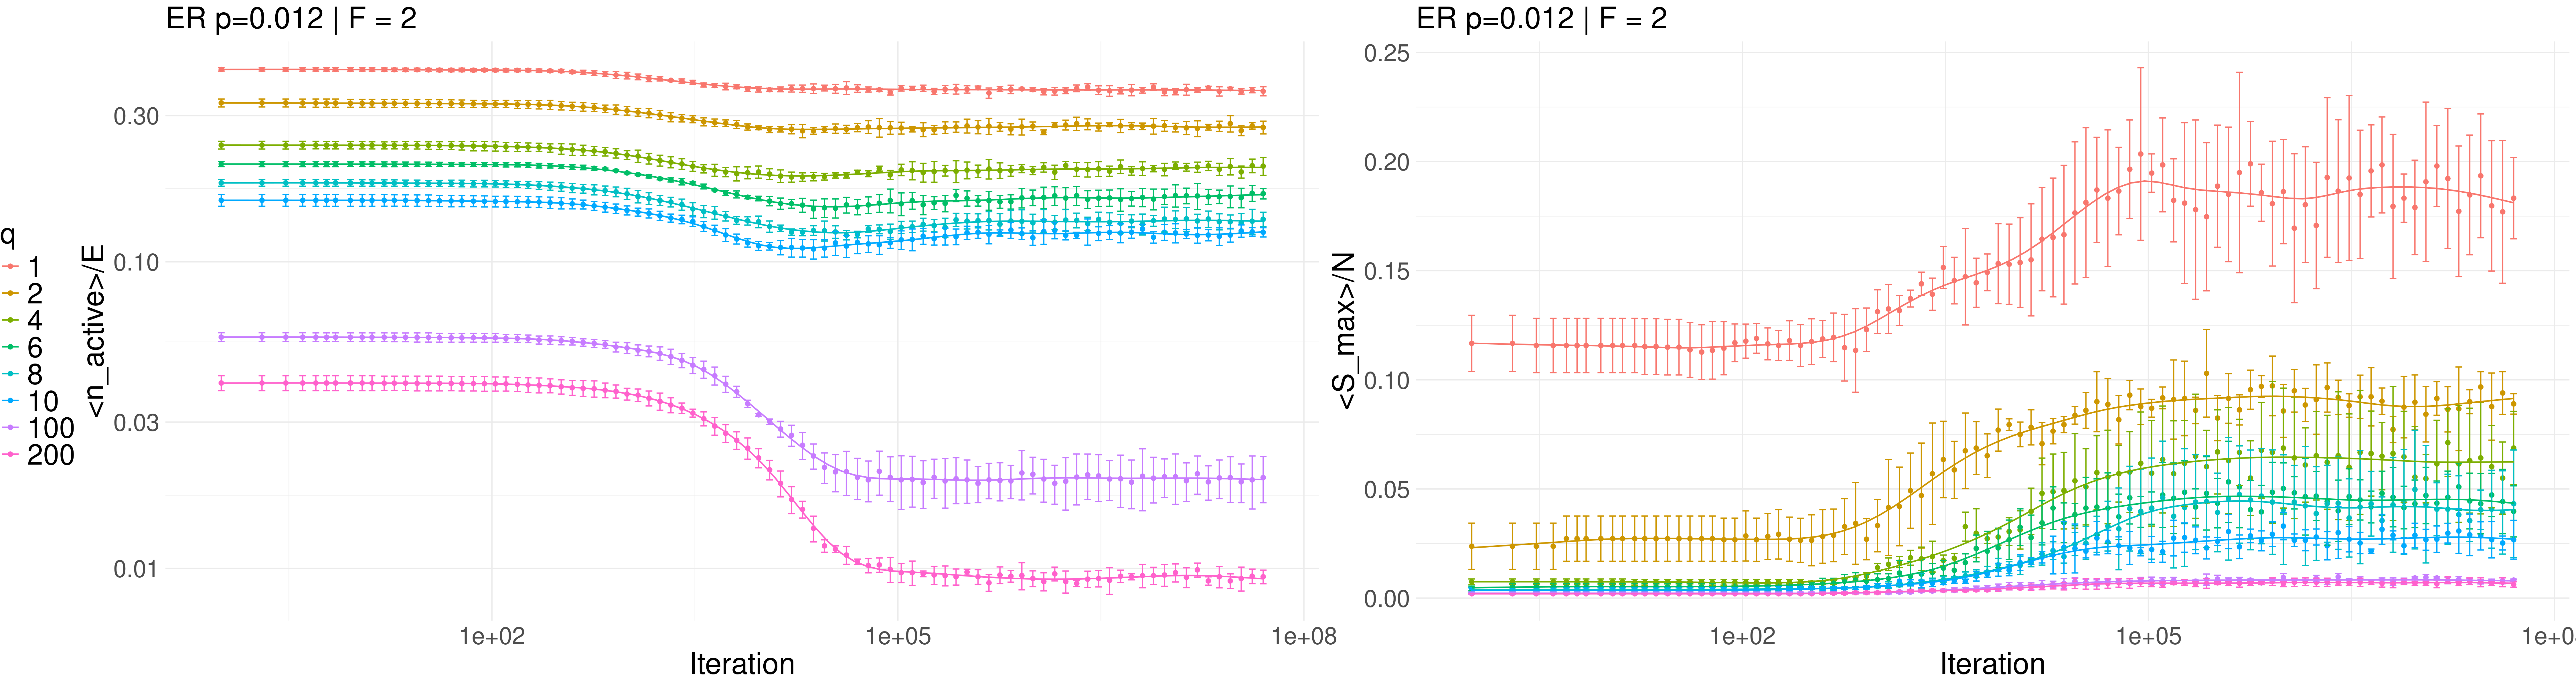
\includegraphics[width=1\textwidth]{images/task30/ER_0-012_2.png} 
    \vspace{-0.5cm}
    \caption{Erdős–Rényi with $p=1.2\times10^{-2}$. $F=2$.} 
\end{figure}


\begin{figure}[h] 
    \centering
    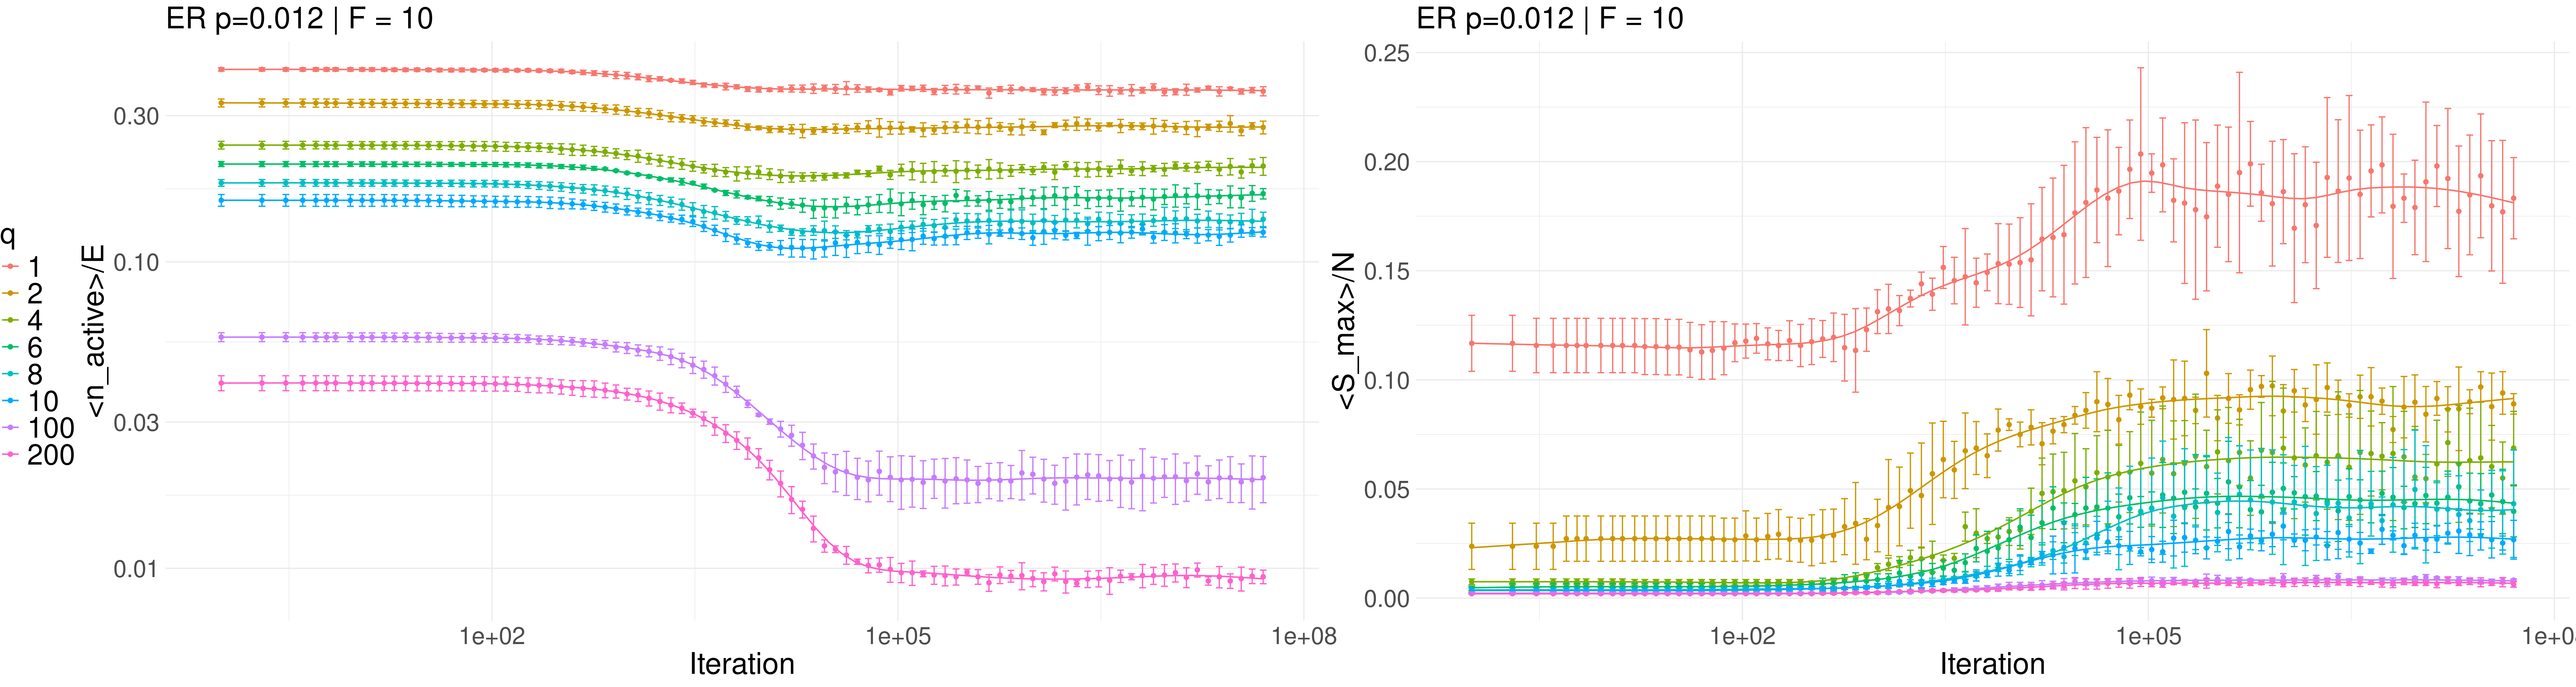
\includegraphics[width=1\textwidth]{images/task30/ER_0-012_10.png} 
    \vspace{-0.5cm}
    \caption{Erdős–Rényi with $p=1.2\times10^{-2}$. $F=10$.} 
\end{figure}

\begin{figure}[h] 
    \centering
    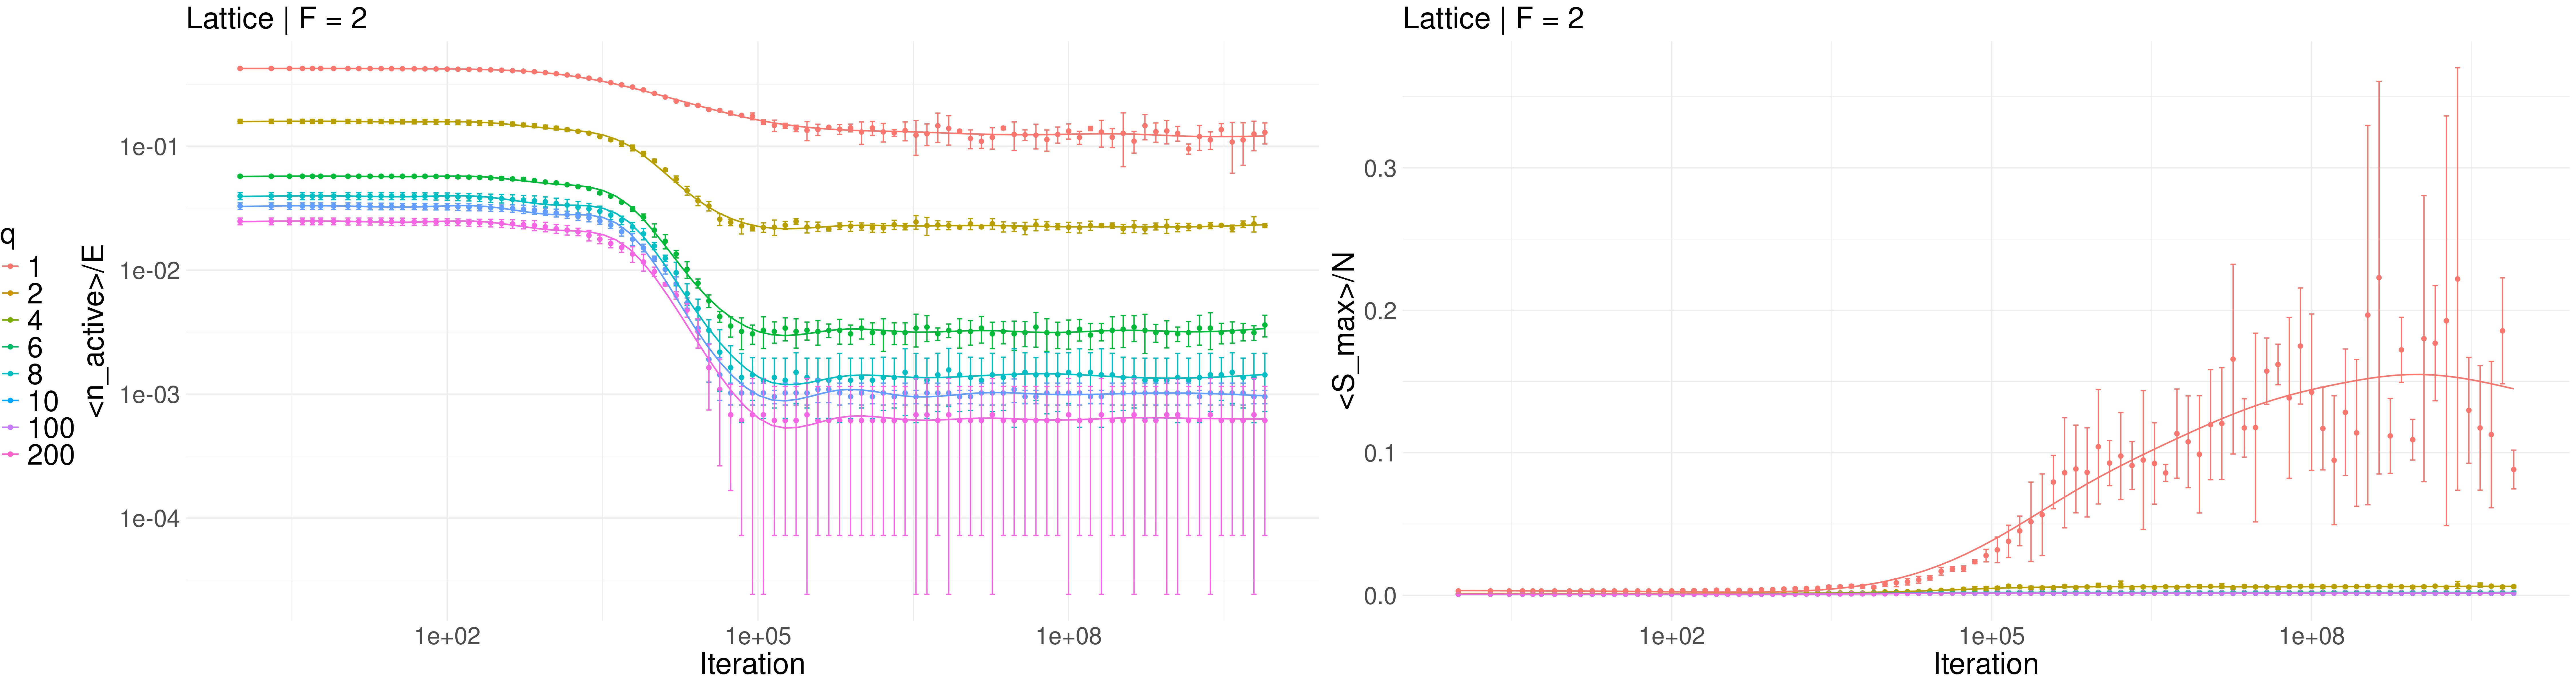
\includegraphics[width=1\textwidth]{images/task30/resultsLattice_2.png} 
    \vspace{-0.5cm}
    \caption{Regular lattice $L=50$. $F=2$.} 
\end{figure}


\begin{figure}[h] 
    \centering
    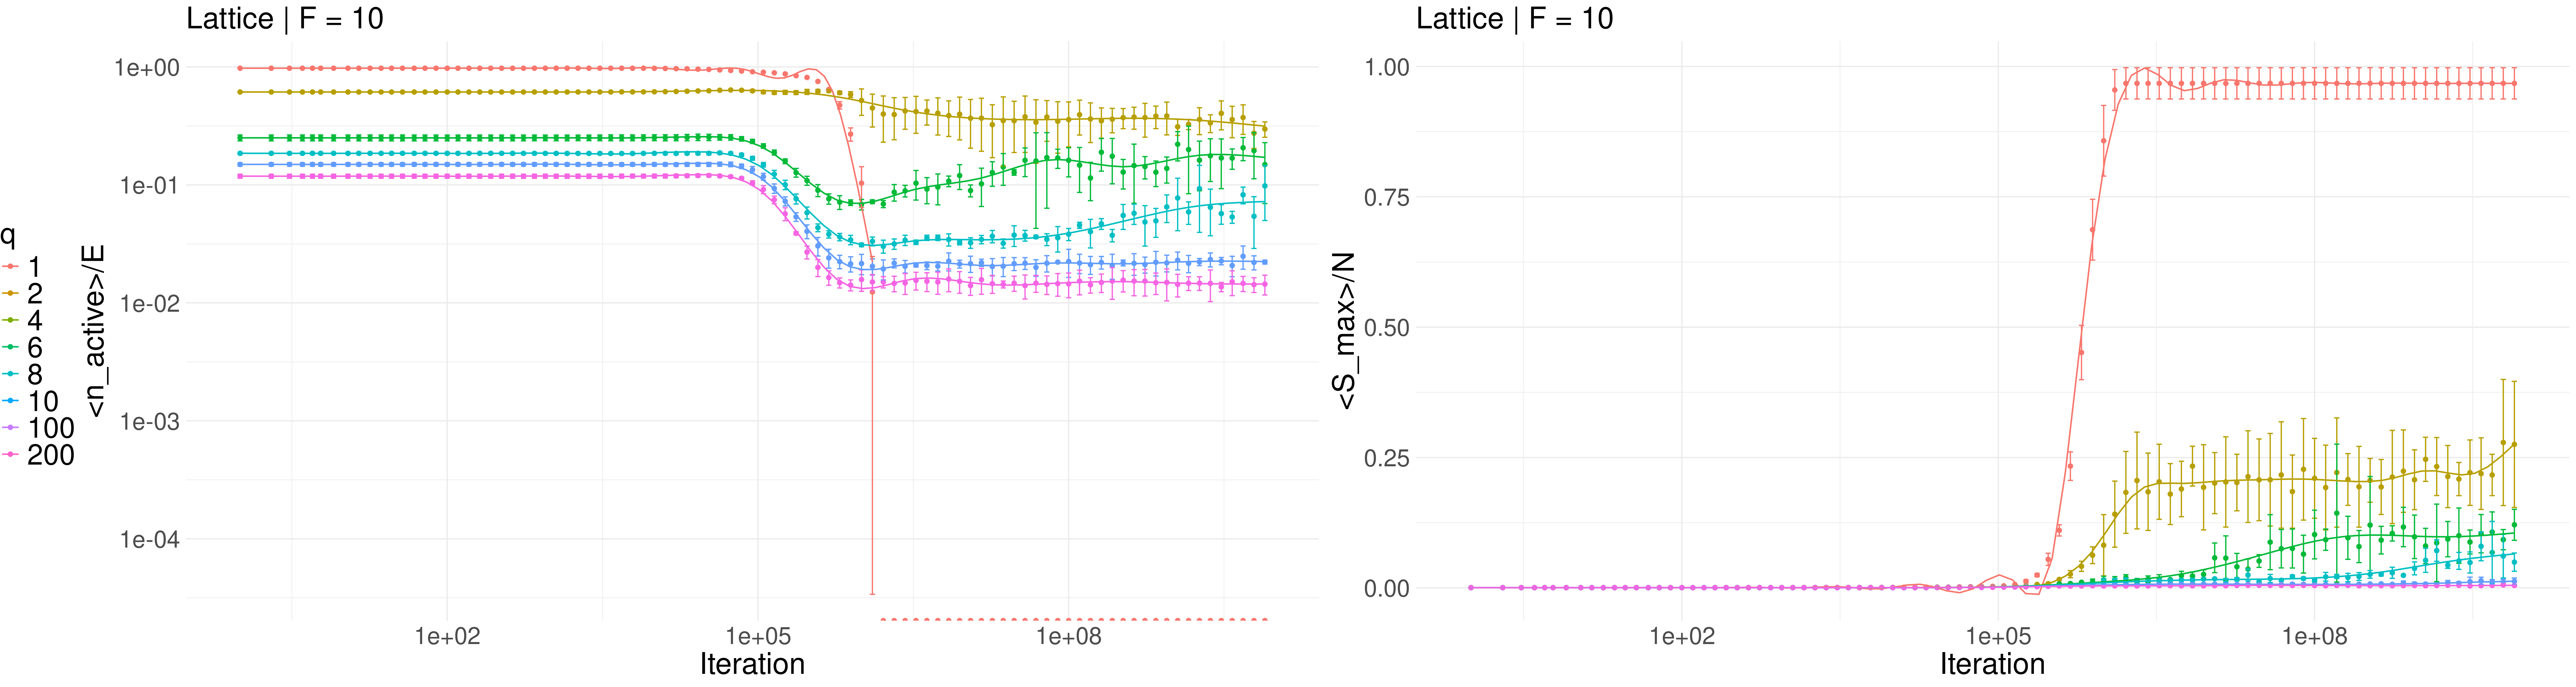
\includegraphics[width=1\textwidth]{images/task30/resultsLattice_10.png}
    \vspace{-0.5cm}
    \caption{Regular lattice $L=50$. $F=10$.} 
\end{figure}


\begin{figure}[h] 
    \centering
    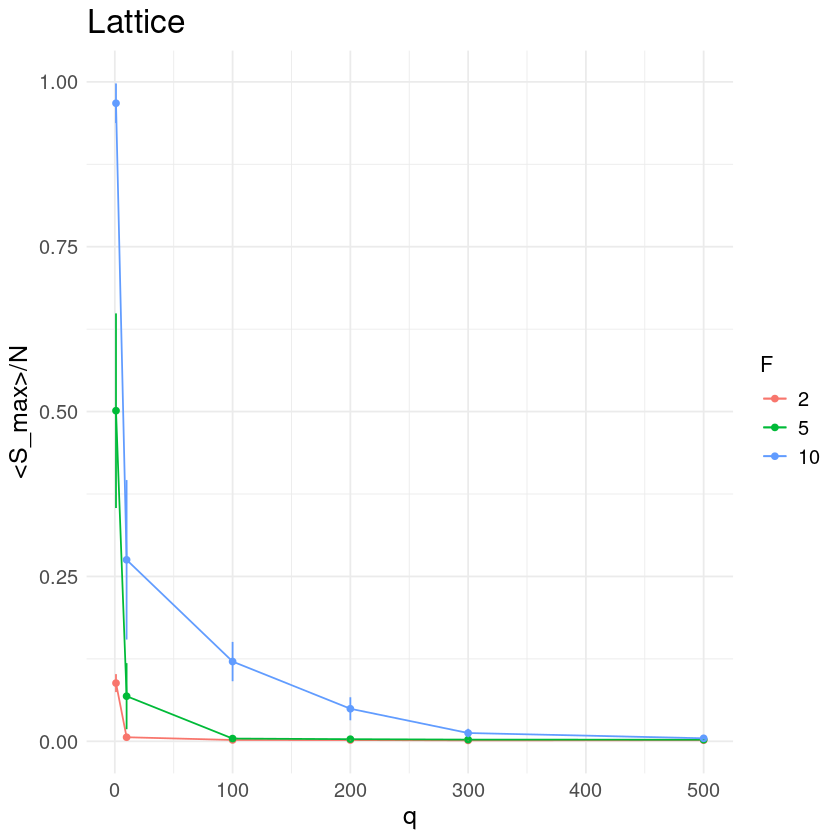
\includegraphics[width=0.5\textwidth]{images/task30/transitionLatice.png} 
    \vspace{-0.5cm}
    \caption{Size of the largest cultural domain after $10^{10}$ iterations as a function of the initial disorder $q$.} 
\end{figure}
